The \verb+vga_drive+ module exists to handle the rendering of a 640x480 resolution image and the bar-graphs on
the vga display. The image beeing rendered consists of a background image previously 
stored in the SRAM consisting of pre filled bars that within the module will be blanked
out according to the input stimuli, which will give the appearance of bars being filled 
to different levels.   

To render an image on the vga screen five main signals is needed. Three analog color channels (red, green and blue)
and two signals for synchronization hsync and vsync. The image is rendered pixel by pixel line by line using
a horizontal sweep pattern which is reset by the two sync signals. If a color is set when the sweep resets
arbitrary patterns can occur and therefore the signal has to be blanked during the reset phase.

The module \verb+vga_drive+ has four input signals described in \ref{tab:input} and five output signals described
in \ref{tab:output} and consists of 11 sub modules which can be overviewed in \ref{fig:vgadrive} and will be described below


\begin{figure}[H]
        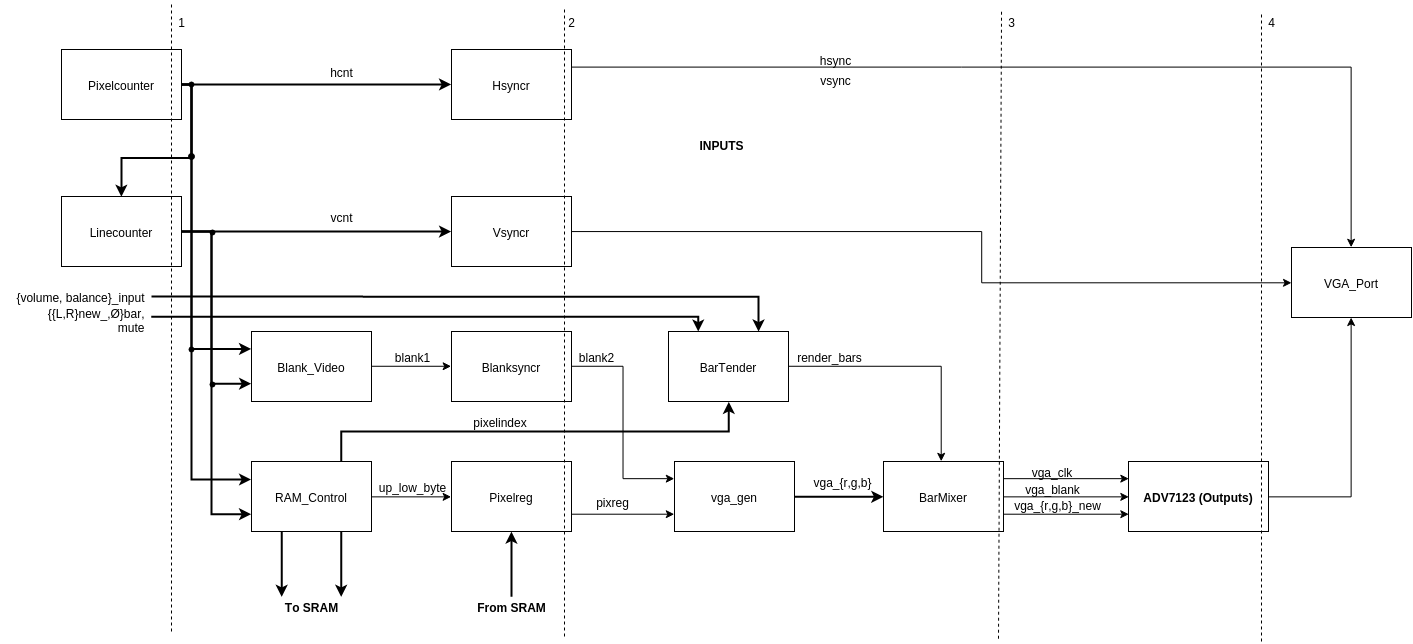
\includegraphics[scale=0.35]{vgadrive.png}
        \caption{Block diagram of vga\_drive}
        \label{fig:vgadrive}
\end{figure}


\begin{figure}[h]
        \caption{List of input signals}
        \label{tab:input}
\begin{tabular}{|r|l|}
        \hline
        \multicolumn{2}{|c|}{Input signals}\\
        \hline
        \multicolumn{1}{|c}{Name} & \multicolumn{1}{c|}{Description} \\
        \hline
        volume\_input & a 4 bit input containing volume information\\
        \cline{1-2}
        \hline
        balance\_input & a 4 bit input containing balance information\\
        \cline{1-2}    
        \hline
        bar & a n bit input containing signal sound input signal level\\
        \cline{1-2}    
        \hline
        new\_bar & a n bit input containing manipulated input signal level\\
        \cline{1-2}    
        \hline
\end{tabular}
\end{figure}

\begin{figure}[h]
        \caption{List of output signals}
        \label{tab:output}
\begin{tabular}{|r|l|}     
        \hline
        \multicolumn{2}{|c|}{output signals}\\
        \hline
        \multicolumn{1}{|c}{Name} & \multicolumn{1}{c|}{Description} \\
        \hline
        vga\_clk & clock signal needed for scanning\\
        \cline{1-2}
        \hline
        vga\_blank & a blanking signal for blanking when resetting scan\\
        \cline{1-2}    
        \hline
        vga\_(r,g,b) & three signals containing color information\\
        \cline{1-2}    
        \hline
\end{tabular}
\end{figure}

\subsection{VGA\_driver:Pipelining}
Since there is a time delay for the system to calculate ram adress, generate pixel\_index the system is
pipelined. The four pipe-line stages is illustrated with dashed lines in figure \ref{fig:vgadrive}.
This means that there is a time delay of 3 clock cycles between which pixel is handled and which is drawn. 

\subsection{VGA\_driver:pixelcounter} 
The sub module \verb+pixelcounter+ is a pixel generating the internal 10 bit signal hcount. hcount
functions as a \verb+pixelcounter+ for each row and will count from 0 to 797 which represent the
pixels needed for each row in the scanning. 
 
\subsection{VGA\_driver:linecounter}
\verb+linecounter+ works almost the same as pixelcounter and generates the signal vcount. vcount is
incremented with one every time hcount resets and resets after reaching 525. This makes hcount and vcount together act as
coordinates to each pixel on the screen during the scanning.

\subsection{VGA\_driver:clock\_divider}
\verb+Clock\_divider+ is just as it's name suggests a clock divider which divides the system clock of 50 MHz
to 25 MHz. This is needed because the timings in the vga-interface for the resolution used 
requires a clock of 25 MHz 

\subsection{VGA\_driver:blank\_video}

Due to the nature of the sweep in the vga-interface the signal needs to be blanked just before,
during and after the syncronization signals. This is done using the blank\_video sub module,
the 1bit blanking signal is active low and should therefore be zero while outside of the visible image and
and one inside. This is done by setting blank high when hsync is between 0 and 639 and vsync is between
0 and 479.    

\subsection{VGA\_driver:RAM\_control}
The image used as a background is pre-stored in the SRAM and to acess the image data we need to generate
some signals to the SRAM. First is the control signals CE, OE, WE, UB, LB which is set constant to
0, 0, 1, 0, 0. Which basically says that SRAM should be enabled read-only and access both upper and lower byte.

Each 16 bit row in the SRAM contains color information about two pixels, one in the lower and one in the upper
byte. Therefore we must generate two signals sram\_addr which provides the SRAM with the correct adress and 
up\_lo\_byte that provides the sub module pixelreg with the information about which of the bytes should be read .
It also generates the output pixelindex which is a counter that counts each pixel in the visible area used
by bar\_tender (more in section \ref{bartender})   

\subsection{VGA\_driver:hsyncr, vsyncr}
The sub modules \verb+hsyncr+ and \verb+vsyncr+ is responsible for generating the hsync and vsync signals used for reseting
the sweep. In the resolution used in this application this means that hsync should be active(low) during 
hcount values between 490 and 493 and vsync between vcount values of 655 and 750.   

\subsection{blank\_syncr}
blank\_syncr is simply a d-flip flop needed for pipelining.

\subsection{VGA\_driver:pixel\_reg}
Pixelregister is responsible for reading the image information from SRAM, the image information is avaliable
on the SRAM-bus and the module simply needs to read the correct byte (using up\_lo\_byte) and put it ine a pipeline
register.

\subsection{VGA\_driver:vga\_gen}
\verb+vga\_gen+ will take the pix\_reg register and supply it to the three color channel outputs 
vga\_r, vga\_g and vga\_b. Due to the fact that the AVD7123 chip expects 10 bit values and the stored image
containing 3bit color values the values need to be scaled up before provided to \verb+bar\_mixer+ 

\subsection{VGA\_driver:bartender and barmixer}\label{bartender}
\verb+bar\_tender+ is the submodule responsible for rendering the bar-graphs displaying volume, balance and
signal strength before and after signal manipulation. The background image already has the bars drawed filled
and to give the apperence of them beeing filled to different levels pixels will be blanked out from the top down. Using the volume, balance, bar, new\_bar and pixelindex \verb+bar\_tender+ will calculate which pixels should
be blanked and set the signal render\_bar high.

\verb+bar\_mixer+ works as a multiplexer blanking out the bars. The color information is passed through if render\_bar signal is low and blanks out the pixel if high which gives the effect of bargraphs beeing filled.
